\documentclass[conference]{IEEEtran}
\IEEEoverridecommandlockouts
\usepackage{cite}
\usepackage{amsmath,amssymb,amsfonts}
\usepackage{algorithmic}
\usepackage{graphicx}
\usepackage{textcomp}
\usepackage{xcolor}
\usepackage{bmpsize}
\usepackage{balance}
\usepackage{float}
\usepackage{enumerate}
\graphicspath{ {./figures/} }
\def\BibTeX{{\rm B\kern-.05em{\sc i\kern-.025em b}\kern-.08em
    T\kern-.1667em\lower.7ex\hbox{E}\kern-.125emX}}

\begin{document}
\title{Towards malware detection based on performance counters using deep learning classification models}

\DeclareRobustCommand*{\IEEEauthorrefmark}[1]{\raisebox{0pt}[0pt][0pt]{\textsuperscript{\footnotesize\ensuremath{
 \ifcase#1\or {*}\or {**}\or {{**}*}\or {{**}{**}}\or 5\or 6\or 7\or 8 \else\textsuperscript{\expandafter\romannumeral#1}\fi}}}}

\author
{
 \IEEEauthorblockN
 {
   Omar Mohamed\IEEEauthorrefmark{1},\IEEEauthorrefmark{2}
 }
 \IEEEauthorblockN
 {
  Ciprian-Bogdan Chirila\IEEEauthorrefmark{2}
 }
 \IEEEauthorblockA
 {\IEEEauthorrefmark{1}Necmettin Erbakan University, Turkey\\
  \IEEEauthorrefmark{2}University Politehnica of Timi\c{s}oara, Romania\\
  Department of Computers and Information Technology\\
  E-mail:
  omar@omarmohamed.com;
  chirila@cs.upt.ro
 }
}

\maketitle

\begin{abstract}
Security exploits and subsequent malware is a challenge for computing systems.

For detecting anomalies and discovering vulnerabilities in computing systems several methods are used: i) malware aware processors; ii) static program analysis; iii) dynamic program analysis.

Malware aware processors require online hardware which is not always a practical and scalable solution.

Static analysis methods imply automated static analysis tools that have a limited performance with
a detection capability that not always meets the requirements of the project regarding the criticality of the application.

Dynamic analysis on the other hand overcame static analysis in latest trends. In this trend performance counters analysis are used in several approaches. 

Operating system performance counters are collected and stored as time series in two contexts: i) in the presence and ii) in the absence of malware.
Ten deep learning models are used for time series classification. 

From the experiments we learned that 2 models are able to detect accurately the presence of malware in an infested operating system, while the rest of the models tend to overfit the data.
\end{abstract}

%\begin{keywords} 
%malware;
%performance counters;
%operating systems;
%program behaviour;
%time series classification;
%deep learning classification models
%\end{keywords}

\section{Introduction}
\label{sec:introduction}
In the context of globalization the physical border security devices of a country do not protect its digital infrastructure. Nowadays security attacks occur at a high rate that are various and complex. It was estimated by antivirus companies that the number of malware is at the size of tens of millions. Malware has a huge rate of growth, namely over 300 new threats are created each minute.
The term of malware denotes malicious software that can damage other software systems.

Companies and state organizations servers are protected by hardware e.g. firewalls, intrusion detection systems (IDS) and software e.g. anti-viruses (AV) solutions.

Hardware protection is usually expensive and thus not always accessible.

The problem with AVs is that in the traditional approach they have static signatures in order to detect malware. Attackers can program malware such that it exhibits benign software signatures. On the other hand AVs are prone to exploits and are consuming a considerable amount of resources so are difficult to use them in real-time protection.

One solution is a detector that classifies programs by identifying malware and then helps applying expensive software based solutions. Such a classification can be made based on logistic regression and neural networks. Hardware classifiers implemented by FPGA malware aware processors are not always practical and scalable.

In this context a malware detector based on the dynamic behaviour of computer programs may overcome the static based detection. The dynamic behaviour is expressed as performance counters time series collected from the operating system.

In this paper we present a framework for training and evaluating deep learning models that detect malware based on performance counters time series classification.

In Figure \ref{fig:approach} we present conceptually our approach.
\begin{figure}[!ht]
\centering
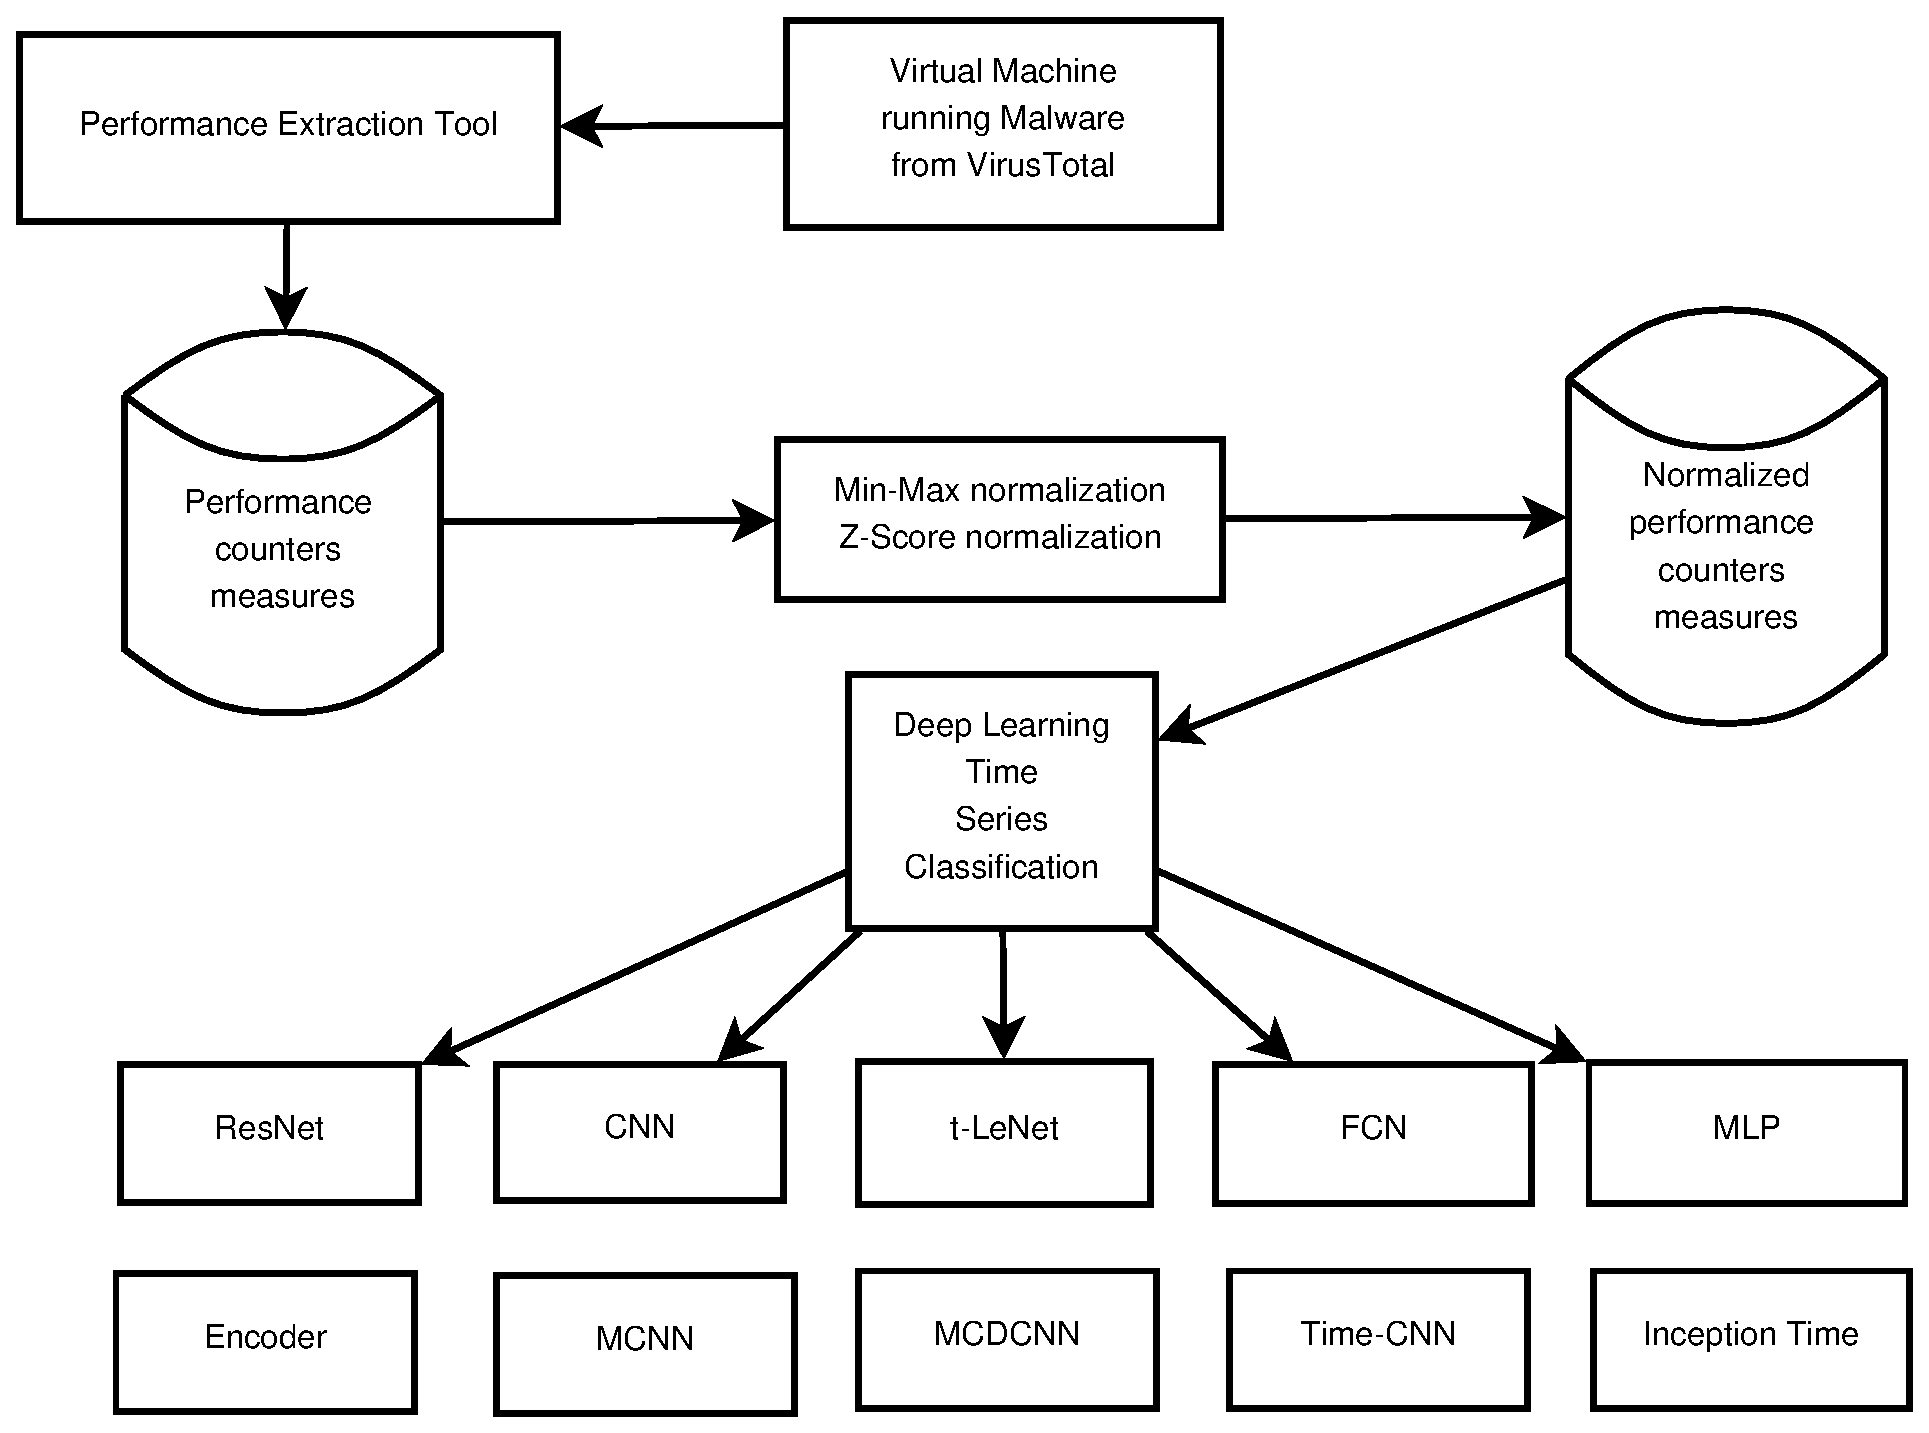
\includegraphics[width=8.5cm]{fig-approach.eps}
\caption{Approach}
\label{fig:approach}
\end{figure}

We start our approach at a Virtual Machine (VM) level running programs in the presence and absence of malware. The malware used in the experiments was obtained from the VirusTotal \cite{VirusTotal2021} company.
On the VM we run in parallel a tool that collects 23 performance counters grouped into time series.
Next, the results are normalized using statistical operators like Min-Max and Z-Score.
On the normalized time series we train 10 deep learning classification models \cite{Fawaz2019}:
\begin{enumerate}[i)]
\item Residual neural network (ResNet);
\item Convolutional Neural Network (CNN);
\item Time Le-Net (t-LeNet);
\item Fully Convolutional Neural Network (FCN);
\item Multi Layer Perceptron (MLP);
\item Encoder;
\item Multi-scale Convolutional Neural Network (MCNN);
\item Multi Channel Deep Convolutional Neural Network (MCDCNN);
\item Time Convolutional Neural Network (Time-CNN);
\item Inception Time.
\item RNN implementaions (LSTM, GRU and vanilla RNN)\cite{azizi2018deep}
\end{enumerate}
On the trained classification models accuracy tests were performed and corresponding graphs were 
plotted. We consider that the trained classifiers could be used on a real machine as a malware detection 
tool.

% paper structure
The paper is structured as follows.
Section \ref{sec:related-works} presents related works in the field of program behaviour analysis 
based on performance counters and deep learning classification models.
Section \ref{sec:experimental-setup} presents the design of the performance counters extraction tool 
and the configuration of the deep learning classification models.
Section \ref{sec:experimental-results} presents the experimental results from the trained 
classification models.
Section \ref{sec:discussion} analyzes the experimental results. 
Section \ref{sec:conclusions-and-future-work} concludes and sets the future work.

\section{Related Works}
\label{sec:related-works}
The work of \cite{Kadiyala2021} is the seminal paper for our approach. They explore performance counters to analyze the behaviour of programs at run-time. They developed a prototype bases on operating system's calls to capture the values of performance counters. Thus, time series are formed describing the behavior of programs in a given period of time. Next, they develop a semi-supervised clustering algorithms to group programs by their intrinsic behaviour. The experiments they carry are based on 18 programs grouped in 4 clusters: web browsers, text editors, image viewers and audio players. They conclude from the experiments that the performance counters accurately differentiate the dynamic behaviour of four clusters of programs. They claim that the results are not influenced by the virtual or physical environment where the programs run.

In \cite{Kundu2021} it is presented a machine learning based approach that optimizes hyper-parameters of machine learning models applied to malware detection problems. Two automated machine learning (AutoML) frameworks are used, namely AutoGluon-Tabular and Microsoft Neural Network Intelligence. They optimize the parameters of Light Gradient Boosted Machine (LightGBM) that is in charge with malware samples classification. In our approach we use other 10 models with no hyper-parameter optimization from \cite{Fawaz2019}.

In \cite{Dinakarrao2019} is presented a hardware-assisted malware detection (HMD) technique using machine learning classifiers. The approach is based on low-level micro-architectural events captured by Hardware Performance Counters (HPC). In the approach they create an adversarial attack on the HMD systems using an adversarial sample predictor. Their intention is to tamper the security by introducing perturbations in the HPC series.

In \cite{Tahir2019} is presented a machine learning approach based on hardware assisted profiling of browser code in real-time. The model classifies unauthorized mining applications even if their code is heavily obfuscated or encrypted.

In \cite{Patel2017} is presented an ML based approach that detect malware based on HPC.

In \cite{Lutsiv2022} is presented a deep semi-supervised learning-based network anomaly detector operating in heterogeneous information systems.

\section{Experimental setup}
\label{sec:experimental-setup}
In this section we will present our experimental setup based on: i) a C\# tool; ii) a Python prototype and iii) 10 deep learning classification models.

\subsection{Testing Environment}\label{sub:TE}
In the experiment we used a virtual machine or cloud machine as we have to execute the malware. 
Such an operation is definitely harmful to run on the working computer.

An Elastic Computing Cloud (EC2) from Amazon Web Services (AWS) \cite{AWS2021} was be used for experimenting. We kept the machine isolated from the Internet, only a specific IP was allowed through the Internet firewall. 

AWS is suitable for testing ransomware which executes normally even without internet connection. In our experiment an Internet connection is required as most malware will not run without connection. So, VirtualBox \cite{VirtualBox2021} was used to create a virtual machine. The machine has installed Microsoft\texttrademark Windows 7 with all required drivers and run-time environments.

\subsection{Performance Counters Extraction Tool (PerfExtract)}\label{sub:PCET}
The PerfExtract tool was developed in C\# as an application that extracts the following counters 
from the Microsoft\texttrademark Windows operating system:
\begin{itemize}
\item \% Privileged Time - percentage of non-idle processor spent executing code in privileged mode;
\item Handle Count - the number of handles currently opened by a process;
\item IO Read Operations/sec - the rate of reads per second for files, network and I/O devices;
\item IO Data Operations/sec - the rate of reads and writes per second for files, network and I/O 
devices;
\item IO Write Operations/sec - the rate of writes per second for files, network and I/O devices;
\item IO Other Operations/sec - the rate of other I/O operations for files, network and I/O devices;
\item IO Read Bytes/sec - the rate of bytes read per second for files, network and I/O devices; 
\item IO Write Bytes/sec - the rate of bytes issued to I/O operations per second for files, network 
and I/O devices;
\item IO Data Bytes/sec - the rate of bytes read and wrote I/O operations per second for files, network and I/O devices;
\item IO Other Bytes/sec - the rate of bytes used in control operations per second for files, network and I/O devices;
\item Page Faults/sec - the rate of page faults per second handled by the processor. It includes both type of page faults: disk page faults and memory page faults;
\item Page File Bytes Peak -  the maximum amount of virtual memory, in bytes, reserved by the target process to be used for paging files; 
\item Page File Bytes - the current amount of virtual memory, in bytes, reserved by the target process to be used for paging files; 
\item Pool Paged Bytes - number of bytes from the area of system memory that can be written to the disk;
\item Pool Non-paged Bytes - number of bytes from the area of system memory that can not be written to the disk;
\item Private Bytes - the size in bytes of the memory allocated that can not be shared with other processes;
\item Priority Base - the current priority base for the target process;
\item Thread Count - the number of threads that are running in the target process;
\item Virtual Bytes Peak - the maximum size in bytes for the virtual address space used by the target process;
\item Virtual Bytes - the size in bytes for the virtual address space used by the target process;
\item Working Set Peak - the maximum size in bytes for the working memory set of the target process;
\item Working Set - the size in bytes of the working memory set for the target process;
\item Working Set Private - subset of working set reflecting the un-shared amount of memory.
\end{itemize}

The time frame for the extraction was set at 30 seconds. The reason for this decision is based on the fact that programs may be used in different scenarios by different users. The startup period is more likely to be the same for most usage scenarios. The acquisition rate was set at 0.5 seconds in order to capture decent length time series.

The PerfExtract tool may be executed using the following syntax:
\begin{verbatim}
perfextract (-f <path to exe file> | 
-p <pid of specific running program>) 
[options] [-o <path to output folder>]
-c Track child processes    
\end{verbatim}

The tool may use the executable image file as an argument or the process identifier.
On the other hand it may track also the child processes of the target process.
The output of the tool is a CSV file containing the time series for each performance counter.

\subsection{Data Preprocessing}\label{sub:DP}
The data is processed by several Python libraries such as pandas, sklearn and numpy. Each data sample dimensionality is 60 x 23, so after loading the whole data set we get a N x 60 x 23 numpy array. The data is getting normalized using min-max normalization:
\[X = \frac{X - X_{min}}{X_{max} - X_{min}}\]
or Z-score normalization:
\[z=\frac{x-\mu}{\sigma}\]
where \(\mu\) is the mean and \(\sigma\) is the standard deviation.

Finally, we split the data set into train, test and validation sets.

\subsection{Deep Learning Classification Models}\label{sub:DLCM}
\paragraph{Residual Neural Network (ResNet)}
The network \cite{Wang2017} is composed of three residual blocks followed by a Global Average Pooling (GAP) layer and a final Softmax layer. 

The classifier number of neurons is equal to the number of classes in a data set. Each residual block is first composed of three convolutions whose output is added to the residual block’s input and then fed to the next layer. 

The number of filters for all convolutions is fixed to 64, with the ReLU (Rectified Linear Unit) activation function that is preceded by a batch normalization operation. In each residual block, the filter’s length is set to 8, 5 and 3.

\paragraph{Convolutional Neural Network (CNN)}
We use a normal Convolutional Neural Network \cite{Krizhevsky2012} with 2 convolution layers and 2 average pooling layers followed by a dense layer with the size of classes' count. 

The convolution layers has a kernel size of 7 and filter sizes of 6 and 12.

\paragraph{Time Le-Net (t-LeNet)}
This model \cite{leguennec:halshs-01357973} can be considered as a traditional CNN with two convolutions followed by a fully connected (FC) layer and a final Softmax layer.

There are two main differences with the FCNs: (1) an FC layer and (2) local maximum pooling operations. For both convolutions, the ReLU activation function is used with a filter length equal to 5. 

For the first convolution, 5 filters are used and followed by a max pooling of length equal to 2. 

The second convolution uses 20 filters followed by a max pooling of length equal to 4. 

The convolutional blocks are followed by a non-linear fully connected layer which is composed of 500 neurons, each one using the ReLU activation function. Finally, we use a Softmax classifier.

\paragraph{Fully Convolutional Neural Network (FCN)}
FCNs are mainly convolutional networks \cite{Wang2017} that do not contain any local pooling layers which means that the length of time series is kept unchanged throughout the convolutions. 

In addition, one of the main characteristics of this architecture is the replacement of the traditional final FC layer with a GAP layer, which reduces drastically the number of parameters in a neural network, while enabling the use of the Class Activation Maps (CAM) that highlights which parts of the input time series contributed the most to a certain classification.

\paragraph{Multi Layer Perceptron (MLP)}
The network \cite{Wang2017} contains 4 layers in total where each one is fully connected to the output of its previous layer.

The final layer is a Softmax classifier, which is fully connected to its previous layer’s output and contains a number of neurons equal to the number of classes in the data set. 

All three hidden FC layers are composed of 500 neurons with ReLU as the activation function. Each layer is preceded by a dropout operation.

\paragraph{Encoder}
Encoder \cite{Sera2018} is a hybrid deep CNN whose architecture is inspired by FCN with a main difference, namely, the GAP layer is replaced with an attention layer. Similarly to FCN, the first three layers are convolutional with some relatively small modifications. 

The first convolution is composed of 128 filters of length 5; the second convolution is composed of 256 filters of length 11; the third convolution is composed of 512 filters of length 21. 

Each convolution is followed by an instance normalization operation whose output is fed to the PReLU (Parametric Rectified Linear Unit) activation function. 

The output of PReLU is followed by a dropout operation and a final max pooling of length 2. 

The third convolutional layer is fed to an attention mechanism that enables the network to learn which parts of the time series are important for a certain classification. 

Finally, a traditional Softmax classifier is fully connected to the latter layer with a number of neurons equal to the number of classes in the data set.

\paragraph{Multi-scale Convolutional Neural Network (MCNN)}
The MCNN architecture \cite{cui2016multiscale} is very similar to a traditional CNN model: with two convolutions (and maximum pooling) followed by an FC layer and a final Softmax layer. 

On the other hand, this approach is very complex with its heavy data pre-processing step. The Window Slicing (WS) method is a data augmentation technique. 

WS slides a window over the input time series and extract subsequences, thus training the network on the extracted subsequences instead of the raw input time series.

\paragraph{Multi Channel Deep Convolutional Neural Network (MCDCNN)}
The architecture \cite{Zheng2014TimeSC} is mainly a traditional deep CNN with one modification for MTS data: the convolutions are applied independently (in parallel) on each dimension (or channel) of the input MTS. 

Each dimension for an input MTS will go through two convolutional stages with 8 filters of length 5 with ReLU as the activation function. 

Each convolution is followed by a max pooling operation of length 2. 

The output of the second convolutional stage for all dimensions is concatenated over the channels axis and then fed to an FC layer with 732 neurons with ReLU as the activation function. 

Finally, the Softmax classifier is used with a number of neurons equal to the number of classes in the data set.

\paragraph{Time Convolutional Neural Network (Time-CNN)}
The first characteristic of Time-CNN \cite{Zhao2017} is the use of the mean squared error (MSE) instead of the traditional categorical cross-entropy loss function. 

The network is composed of two consecutive convolutional layers with respectively 6 and 12 filters followed by a local average pooling operation of length 3. 

The convolutions adopt the sigmoid as the activation function. 

The network’s output consists of an FC layer with a number of neurons equal to the number of classes in the data set.

\paragraph{Inception Time}
This classifier \cite{Fawaz2020} is built of 2 residual blocks, each block contains 3 inception modules instead of fully connected layers. 

Each block's output is transferred using a shortcut layer to the next block's input. 

After the residual blocks a Global Average Layer in used and finally a fully connected layer with Softmax function and a number of neurons equal to class the number of classes.
\paragraph{RNN}
LSTM, GRU, and simple RNN classifiers implemented by Shekoofeh Azizi\cite{azizi2018deep}

\section{Experimental results}
\label{sec:experimental-results}
In this section we will present the experimental results obtained for each of the deep learning classification models.
\begin{figure}[H]
  \centering
  \begin{minipage}[b]{4.25cm}
    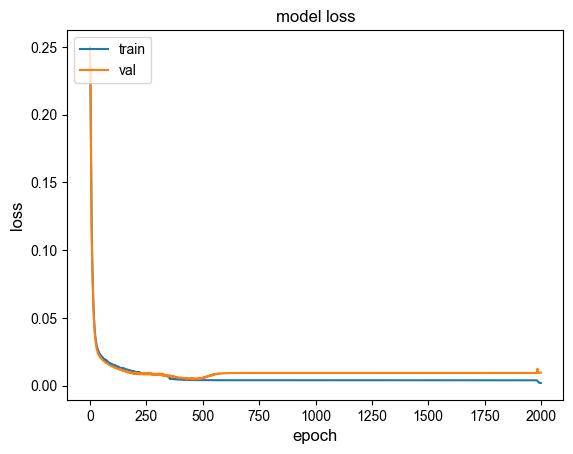
\includegraphics[width=4.25cm]{cnnepochs_loss}
    \caption{CNN}
    \label{fig:cnn}
  \end{minipage}
  \hfill
  \begin{minipage}[b]{4.25cm}
    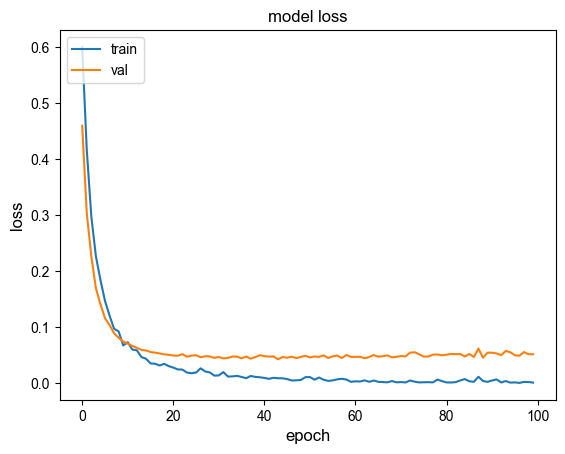
\includegraphics[width=4.25cm]{encoderepochs_loss}
    \caption{Encoder}
    \label{fig:encoder}
  \end{minipage}
\end{figure}

\begin{figure}[H]
  \centering
  \begin{minipage}[b]{4.25cm}
    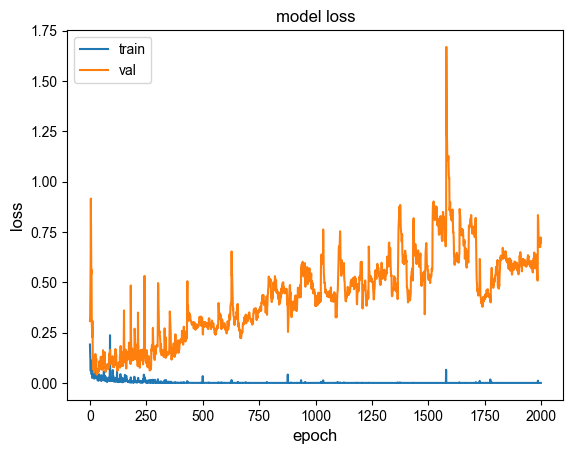
\includegraphics[width=4.25cm]{fcnepochs_loss}
    \caption{FCN}
    \label{fig:fcn}
  \end{minipage}
  \hfill
  \begin{minipage}[b]{4.25cm}
    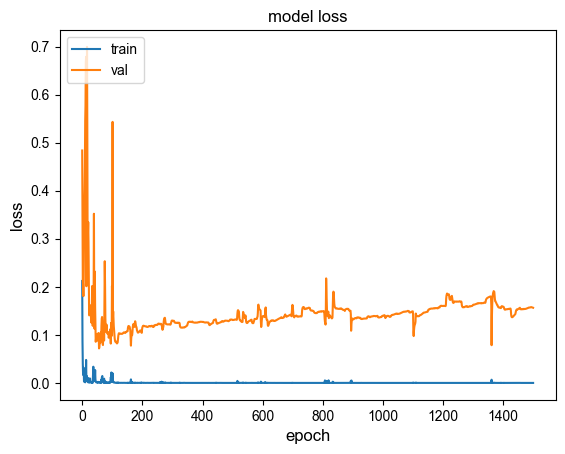
\includegraphics[width=4.25cm]{inceptionepochs_loss}
    \caption{Inception Time}
    \label{fig:inception}
  \end{minipage}
\end{figure}

\begin{figure}[H]
  \centering
  \begin{minipage}[b]{4.25cm}
    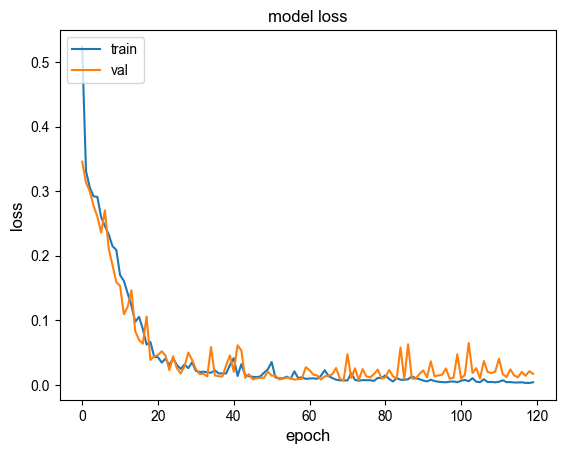
\includegraphics[width=4.25cm]{mcdcnnepochs_loss}
    \caption{MCDCNN}
    \label{fig:mcdcnn}
  \end{minipage}
  \hfill
  \begin{minipage}[b]{4.25cm}
    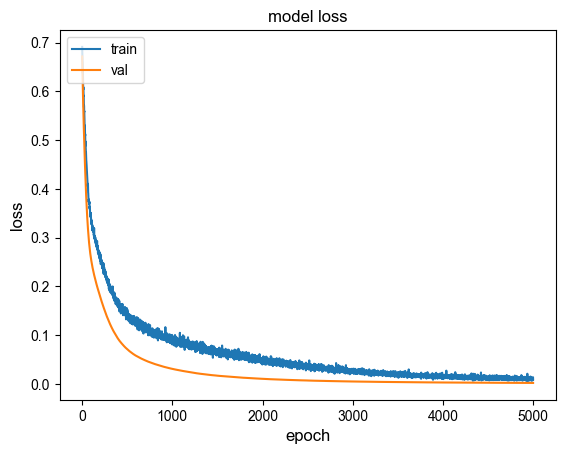
\includegraphics[width=4.25cm]{mlpepochs_loss}
    \caption{MLP}
    \label{fig:mlp}
  \end{minipage}
\end{figure}

\begin{figure}[H]
  \centering
  \begin{minipage}[b]{4.25cm}
    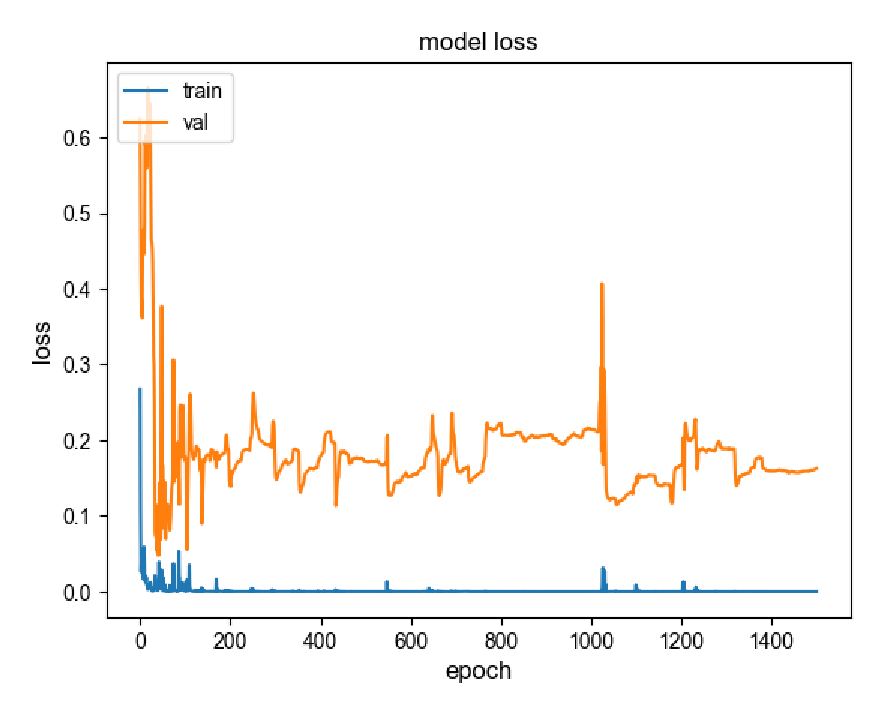
\includegraphics[width=4.25cm]{resnetepochs_loss}
    \caption{ResNet}
    \label{fig:resnet}
  \end{minipage}
  \hfill
  \begin{minipage}[b]{4.25cm}
    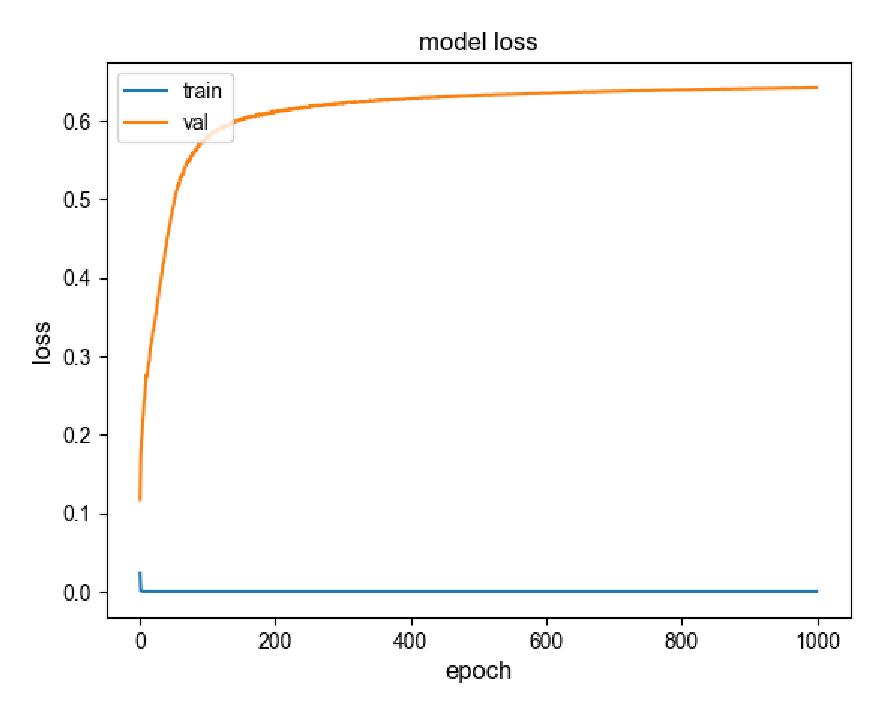
\includegraphics[width=4.25cm]{tlenetepochs_loss}
    \caption{t-LeNet}
    \label{fig:tlenet}
  \end{minipage}
\end{figure}

\begin{figure}[H]
  \centering
  \begin{minipage}[b]{4.25cm}
    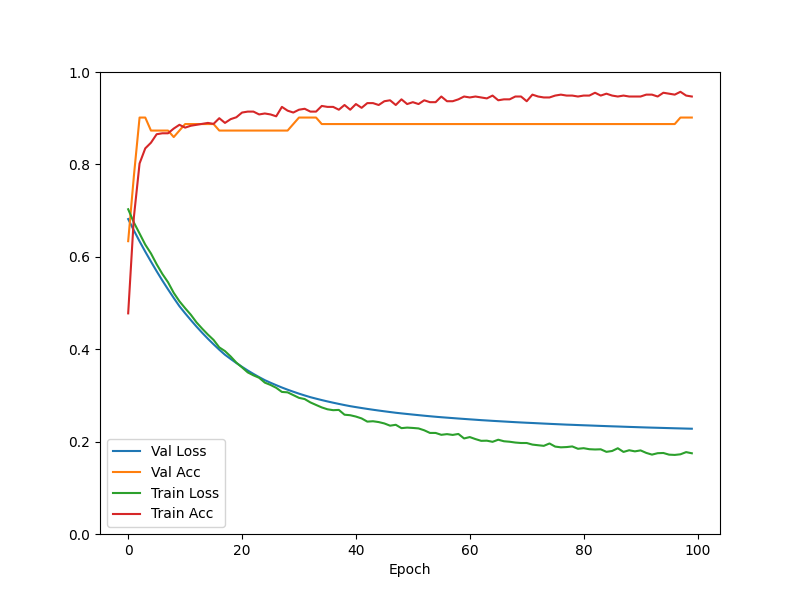
\includegraphics[width=4.25cm]{2lstm}
    \caption{2 LSTM + Dense}
    \label{fig:2lstm}
  \end{minipage}
  \hfill
  \begin{minipage}[b]{4.25cm}
    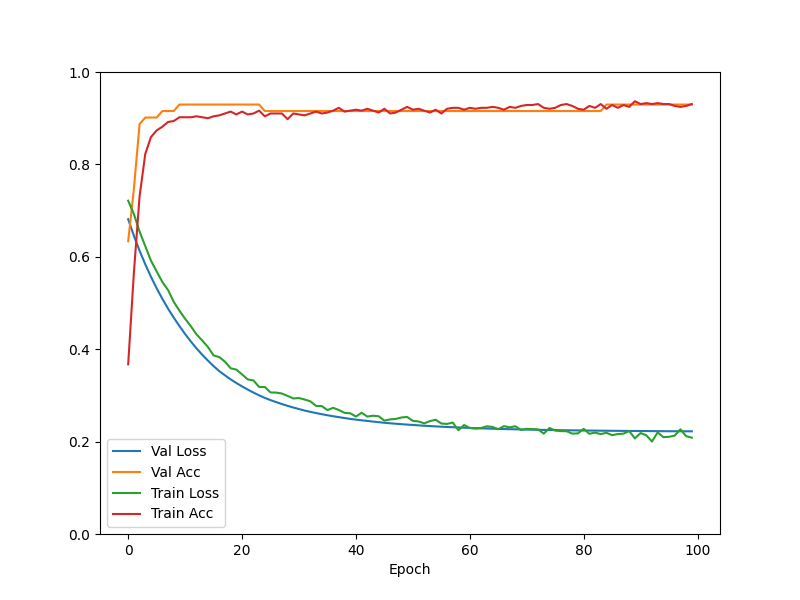
\includegraphics[width=4.25cm]{2gru}
    \caption{2 GRU + Dense}
    \label{fig:2gru}
  \end{minipage}
\end{figure}

\begin{figure}[H]
  \centering
  \begin{minipage}[b]{4.25cm}
    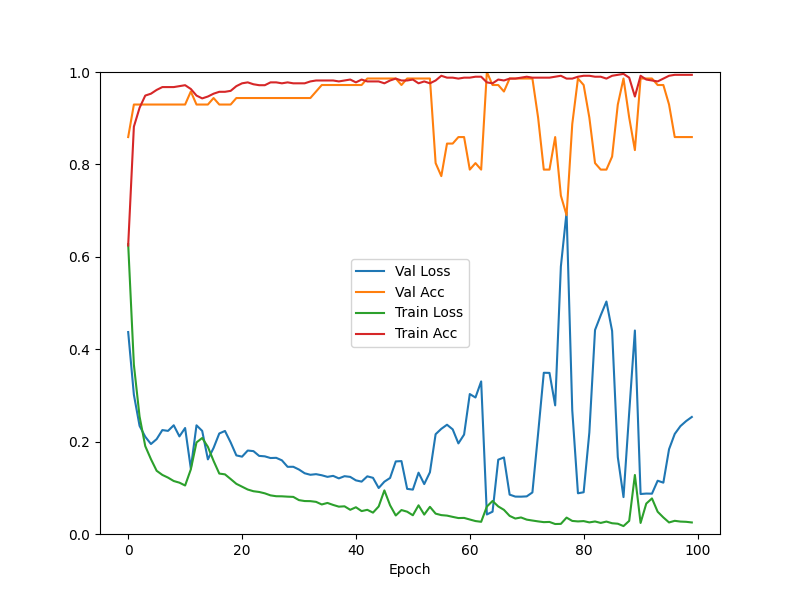
\includegraphics[width=4.25cm]{2rnn}
    \caption{2 RNN + Dense}
    \label{fig:2rnn}
  \end{minipage}
  \hfill
  \begin{minipage}[b]{4.25cm}
    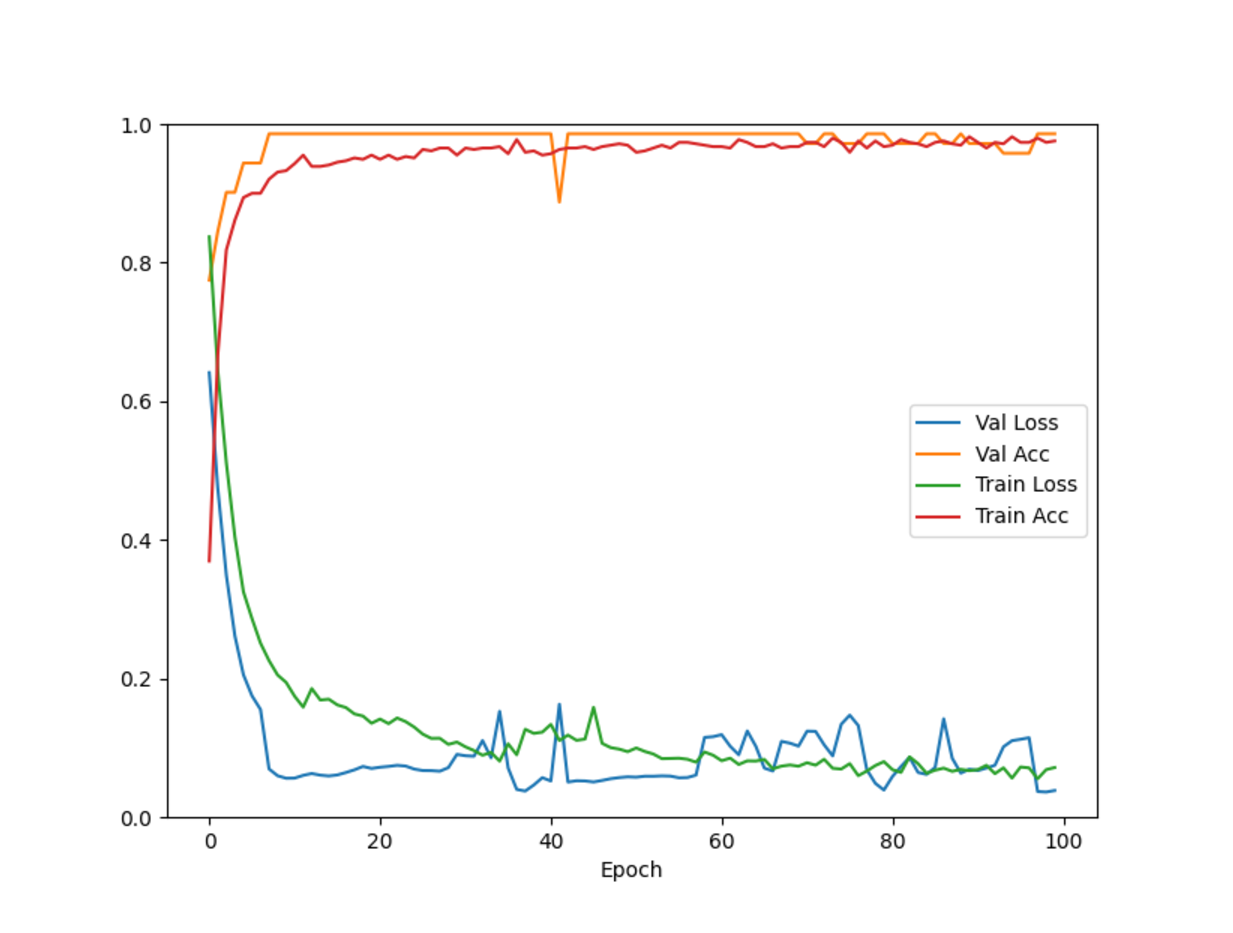
\includegraphics[width=4.25cm]{1rnn}
    \caption{1 RNN + Dense}
    \label{fig:1rnn}
  \end{minipage}
\end{figure}


By looking at figures \ref{fig:fcn}, \ref{fig:inception}, \ref{fig:tlenet} and \ref{fig:resnet} we can see that these models tend to over-fitting, especially t-LeNet (Fig. \ref{fig:tlenet}) model. 

The MCNN model failed with 58\% accuracy, 50\% recall, 29\% precision and 0.37 f1 score. 

MLP (Fig. \ref{fig:mlp}) and CNN (Fig. \ref{fig:cnn}) models over-fitted with 100\% accuracy, and precision, recall, and f1 score of 1. 

Encoder and MCDCNN (Fig. \ref{fig:mcdcnn}) models performed well even with our small data set with a 98\% accuracy, 97\% recall and precision, and 0.97 f1 score. 

FCN, Inception and ResNet models' performance can be improved by using more complex data pre-processing techniques and increasing the data set size. 

In Fig. \ref{fig:2lstm}. a RNN implementation consists of 2 LSTM layers and 1 Dense layer was tested and resulted in 90\% validation accuracy.

In Fig. \ref{fig:2gru}. a RNN implementation consists of 2 GRU layers and 1 Dense layer was tested and resulted in 93\% validation accuracy.

In Fig. \ref{fig:2rnn}. a RNN implementation consists of 2 simple RNN layers and 1 Dense layer was tested and resulted in 100\% validation accuracy.

In Fig. \ref{fig:1rnn}. a RNN implementation consists of 1 simple RNN layer and 1 Dense layer was tested and resulted in 98\% validation accuracy.

The overall performance of all the models definitely will be improved after increasing the data set size.
\begin{center}
\begin{tabular}{||c c c c c||} 
 \hline
 Model & val\_acc & precision & recall & f1 \\ [0.5ex] 
 \hline\hline
 CNN & 0.99 & 0.991 & 0.989 & 0.99 \\ 
 \hline
 Encoder & 0.985 & 0.981 & 0.974 & 0.977 \\
 \hline
 FCN & 0.9 & 0.907 & 0.909 & 0.908 \\
 \hline
 Inception & 0.985 & 0.985 & 0.986 & 0.985 \\
 \hline
 MCDCNN & 0.981 & 0.979 & 0.979 & 0.979 \\ 
 \hline
 MCNN & 0.589 & 0.294 & 0.5 & 0.37 \\ 
 \hline
 MLP & 1 & 1 & 1 & 1 \\
 \hline
 ResNet & 0.976 & 0.973 & 0.975 & 0.974 \\
 \hline
 t-LeNet & 0.987 & 0.984 & 0.986 & 0.985 \\
 \hline
 TWIESN & 0.985 & 0.988 & 0.982 & 0.985 \\ 
 \hline
  2 LSTM & 0.901 & 0.891 & 0.953 & 0.921 \\
 \hline
 2 GRU & 0.929 & 0.913 & 0.976 & 0.943 \\
 \hline
 2 RNN & 1 & 1 & 1 & 1 \\
 \hline
 1 RNN & 0.985 & 1 & 0.976 & 0.988 \\ 
 \hline
\end{tabular}
\end{center}

\section{Discussion}
\label{sec:discussion}
The results are affected by 2 major factors, data samples number and the similar processes. 

Apparently, our dataset consisting of 700 samples wasn't enough for some classifiers and led to overfitting. 

The second problem is the malware downloader and the fake processes that create the main malware process. 

These processes are very similar in terms of counters' data to a lot of legitimate windows services' processes and some other processes like auto updaters. 

We can see that this problem affected FCN, t-LeNet, ResNet, and FCN networks as they couldn't differentiate between these processes in the validation set. 

This problem can be solved by using different approaches in the counters extraction process like identifying the processes that cause the problem and ignoring them so that we end up only with the effective and real processes. 

Also increasing the size and variety of the data set will be very effective. 

Despite these problems, a couple of models achieved a promising results.

\section{Conclusions and Future Work}
\label{sec:conclusions-and-future-work}
In this paper we presented an experimental setup where performance counters time series were 
extracted from a safe and a malware infected virtual machine obtained from VirusTotal.

The performance counter time series were normalized and were used to train 10 deep learning classification models.

Encoder and MCDCNN models gave the best result, while the other models tended to overfit.

As future work we intend to test more malware and to increase the data set size to avoid overfitting problems.

A different malware categories will be tested to increase the variation of the data set and try to mimic a real-time anti-virus.

\section*{Acknowledgment} 
This paper was partially supported by a grant of the Romanian Ministry of Research, Innovation and Digitization, 
project number POC\/398\/1-Development of networks of R\&D centers, 
coordinated at national level and connected to European and international networks and 
ensuring researchers’ access to European and international scientific publications and databases, 
entitled “High Performance Cloud Platform at Politehnica University of Timisoara”, SMIS 123466.

\bibliographystyle{plain}
\balance
\bibliography{bibliography}
\end{document}
